\section{Background and Related Work}
Our work lies at the intersection of embodied vision-language navigation, structured $3$D spatial memory, spatial reasoning with multimodal foundation models, and probabilistic grounding. We review the most relevant directions and highlight the gaps our method addresses. %\opnote{like you said earlier, this section is too big right now. We should condense it to a page max. The way you do it like you hinted last time is to make a general/common statement followed by multiple citations, and not talk about each paper/work individually. your job in this, ironically, is not to educate but to complain about related works and argue conceptually that you are better/similar/different.}

%\tn{If you can reduce each subsection to a paragraph then you don't even need the subsections} 
\noindent{\textbf{{Embodied Question Answering and Vision-Language Navigation:}}}
Embodied Question Answering (EQA) and Vision-and-Language Navigation (VLN) both require an agent to ground language into actions over long horizons under partial observability, using only egocentric observations~\cite{das2018embodiedqa}.
Many embodied systems still commit to a single action or discrete target at each step, so early grounding errors compound and can derail the entire trajectory \cite{cohen2024surveyroboticlanguagegrounding,ahn2022saycan, dai2024thinkactaskopenworld}.
Some prior VLN-based works explicitly identify this issue and introduce backtracking and progress-based recovery to mitigate trajectory drift under greedy decisions~\cite{ma2019regretful}.
Conceptually, our approach addresses the same failure mode by shifting goal grounding to producing a planner-ready goal representation in a generated map rather than a one-shot action choice.
% , so that planning and execution can be driven by a geometric target distribution rather than by a one-shot action choice.
% \opnote{tie it back to your project. How does your work connect to long horizon planning?}
%\tn{cut: Our setting matches this regime, but focuses on a failure point that becomes dominant in long-horizon behavior: repeatedly converting a language goal into an executable target in a consistent $3$D frame. Even when a policy can explore and maintain state, metric-semantic queries demand geometric and spatial consistency that must remain stable as the viewpoint changes and map evolves.}
%\opnote{say how you solve this problem conceptually}\ljnote{fixed}

\noindent{{\textbf{Structured $3$D Spatial Memory and Scene Graphs:}}}
%\tn{I'd either cut this entire subsection or just say the $3$D scene graphs are useful and an input to our system, but alone they cannot produce planner-ready navigation goals.} 
Embodied reasoning benefits from having an explicit spatial memory that persists across time and supports queries about objects, places, and their relations. Hydra~\cite{hydra}, along with Kimera~\cite{rosinol2020kimeraopensourcelibraryrealtime} construct and optimize an online $3$D scene graph that unifies metric layers (e.g., distance fields), object nodes, and higher-level place and room structure~\cite{hydra}.
However, scene graphs cannot produce planner-ready navigation goals as they contain only adjacency information while lacking metric information about a physical space. We therefore build on Scene Graphs a spatial backbone over which metric-semantic language can be composed into planner-ready target distributions (see Fig. \ref{fig:method-overview}).

%\tn{That's why we use.../state how this ties into our work (do we need this para? they're relevant but not directly, maybe shorten and put in experiment details? if you keep it then need to better explain why hydra/kimera alone cannot solve our problem)}
%\opnote{don't go over one paragraph without connecting it to your work. How do you use this? Why is it important to state here?} \ljnote{fixed}
 %\opnote{this paragraph is misplaced. Perhaps have it in the intro or methods.}\ljnote{removed para, we have similar in intro}
%Scene graphs have also been adopted as a memory substrate for embodied goal reasoning  and planning~\cite{graphEQA,vlmap,Ray24arxiv-tamp}.
\noindent\textbf{Spatial Reasoning Limits of Multimodal Foundation Models:}
%\spnote{write about how some specialist reasoners have fined tuned their models spatial reasoner with reasoning traces to introduce how spatial transformation calculation is done, but the fundamental flaw is that they do it in a predefined frame of reference ( world coordinates) and true solution extends into continuous world than the world they build from a single image, so they aren't enough to solve the entire query reliably, they }
Although LLMs and VLMs are strong on many language tasks, their spatial competence remains inconsistent~\cite{vsiBench,frameOfReferenceAmbiguity,spatialRGPT, 3dsrbench}. Across evaluations, common failure modes include unstable visual distance estimates, inconsistent camera framing, and lack of mechanisms to ground visual information \cite{frameOfReferenceAmbiguity, 3dsrbench}.
Several works attempt to address these issues through spatial fine-tuning or by incorporating depth, but the gap  remains for embodied settings where the agent must maintain a consistent allocentric representation over time~\cite{vsiBench,spatialRGPT, 3dsrbench}. Our approach addresses these limitations at the interface level by making the spatial target explicit within a metric semantic map.
% and map-aligned by grounding referents using foundation models as spatio-visual experts in a persistent $3$D scene graph, expressing metric and directional intent as analytic continuous kernels composed into \(P(x)\).
%\opnote{always connect all paragraphs in the related works section back to why your method is better- conceptually. Like how do you conceptually overcome the problem you just state through your methods- no details.}


\noindent\textbf{Vision-Language-Action Models and Affordance Learning:}
Vision-language-action (VLA) models learn end-to-end policies from multimodal inputs to actions, and large-scale training has shown strong transfer, with navigation-focused variants improving robustness through flexible goal conditioning on language, goal images, or goal poses \cite{openx2023rtx,hirose2025omnivla}. However, these policies are typically trained to predict actions rather than to explicitly infer a metric goal in a shared $3$D frame. Our work is novel in that it creates compositional interfaces between a planning or navigation stack, a semantic perception stack, and a mapping stack to generate actions. 
% This motivates goal interfaces that remain map-based and planner-compatible, even when learned components are used for perception or high-level conditioning. These VLA systems do not directly target controlled composition of multi-clause spatial constraints, which is central to instructions that combine multiple relations or additional metric qualifiers, this is demonstrated by Poco \cite{poco}.
%\opnote{why should they? complain about things like accuracy/lack of spatial awareness etc.}.

\noindent{\textbf{{Probabilistic Grounding and Multi-Expert Fusion:}}}
Grounding language in the physical world has long been treated as probabilistic inference, where linguistic structure induces latent grounding variables over referents, relations, and actions \cite{tellex2011symbolgrounding, ijcai2018p810}. This formulation is
%particularly
well suited to spatial language, where predicates such as ``left of'' or ``near'' define distributions over regions of space rather than point locations. A complementary theme is decomposing a complex task into reusable parts to generalize better than monolithic policies when the combinatorics grow \cite{poco, patil2025factorizingdiffusionpoliciesobservation, du2024compositionalgenerativemodelingsingle}. To combine multiple information sources, products of experts (PoE) offer a principled mechanism that multiplies distributions and renormalizes, producing solutions that satisfy multiple constraints simultaneously \cite{hinton2002poe}. Finally, recent embodied systems increasingly combine multiple models or signals, such as mixing perception with language reasoning or fusing goal proposals with feasibility checks \cite{rana2023sayplan}.


%\paragraph{Products of Experts and Agentic Reasoning Loops}
%\tn{cut/merge with above: Products of Experts (PoE) combine multiple constraints by multiplying expert distributions and renormalizing, which encourages agreement regions and is especially natural when each expert encodes a different aspect of the goal \cite{hinton2002poe}. In log space, this corresponds to adding expert energies, closely mirroring how spatial constraints can be composed from independent kernels. Separately, recent agentic frameworks for LLMs emphasize iterative reasoning loops that interleave structured decisions with environment interaction and self-correction, improving reliability under partial observability \cite{yao2022react,shinn2023reflexion}. These ideas motivate organizing goal grounding as a modular loop where intermediate hypotheses (referents, frames, and spatial constraints) can be validated and revised before committing to execution.}


Our work builds on these directions by addressing the missing interface between structured $3$D spatial memory and planner execution for metric-semantic queries, providing a map-aligned and controllable mechanism for translating language into navigation targets (see Fig. \ref{fig:method-overview}).
\begin{figure*}
    \centering
    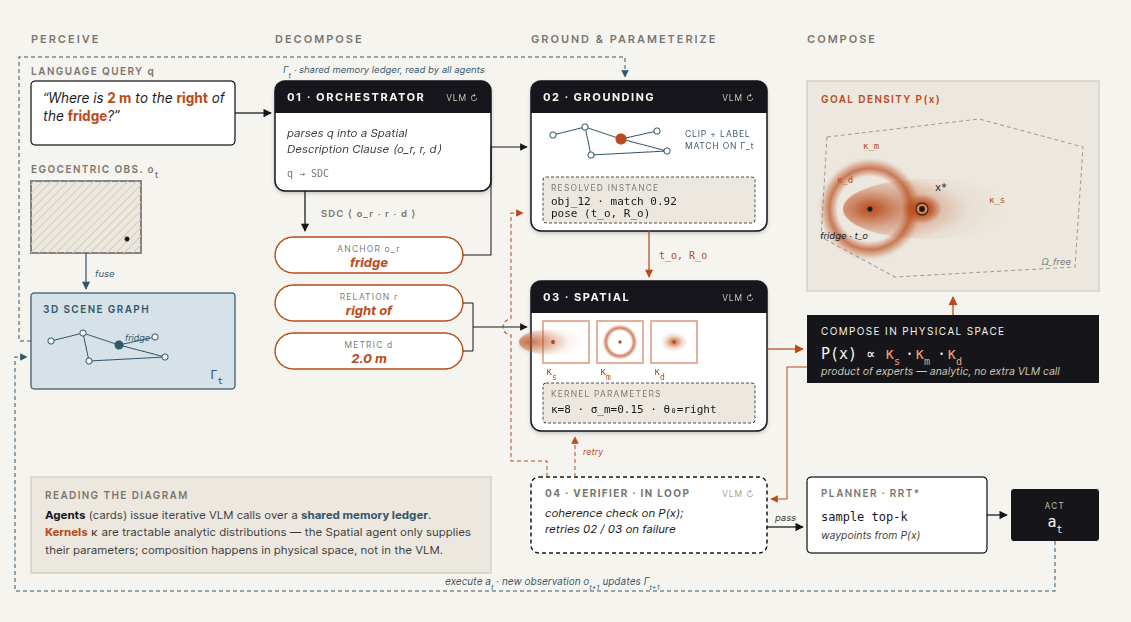
\includegraphics[width=0.99\linewidth]{figures/fig_3_system_overview.png}
    \caption{
      \textbf{MAPG system overview.}
      Egocentric observations $o_t$ are fused into a $3$D scene graph $\Gamma_t$, shared by all agents over a memory ledger.
      The Orchestrator parses the query $q$ into a Spatial Description Clause $\langle o_r, r, d\rangle$; the Grounding Agent resolves the referent $o_r$ against $\Gamma_t$; the Spatial Agent supplies parameters for the directional ($\kappa_s$), metric ($\kappa_m$), and anchor-density ($\kappa_d$) kernels.
      The kernels are composed analytically in physical space (a product of experts, no extra VLM call), yielding a goal density $P(x)$ over free space.
      The Verifier checks coherence and triggers corrective retries; on pass, the Planner samples top-$k$ waypoints to act, and the new observation updates $\Gamma_{t+1}$, closing the loop. \opnote{empty space}
      % \opnote{While I appreciate the effort, I'm not a fan of this figure. Can you please look at Figure 3 in GraphEQA paper and think if you can redesign this one similarly? Remember that your job through the image is not to convey the complexity of your method in its full glory, but to differentiate your method schematically from existing ways. Also you don't even talk about the verifier in your methods section. Perhaps also use this diagram to differentiate what you call an agent and what is a kernel.}
    }
    \label{fig:method_overview-h}
\end{figure*}


